\section{Circuit}
The circuit schematic is as follows:\\
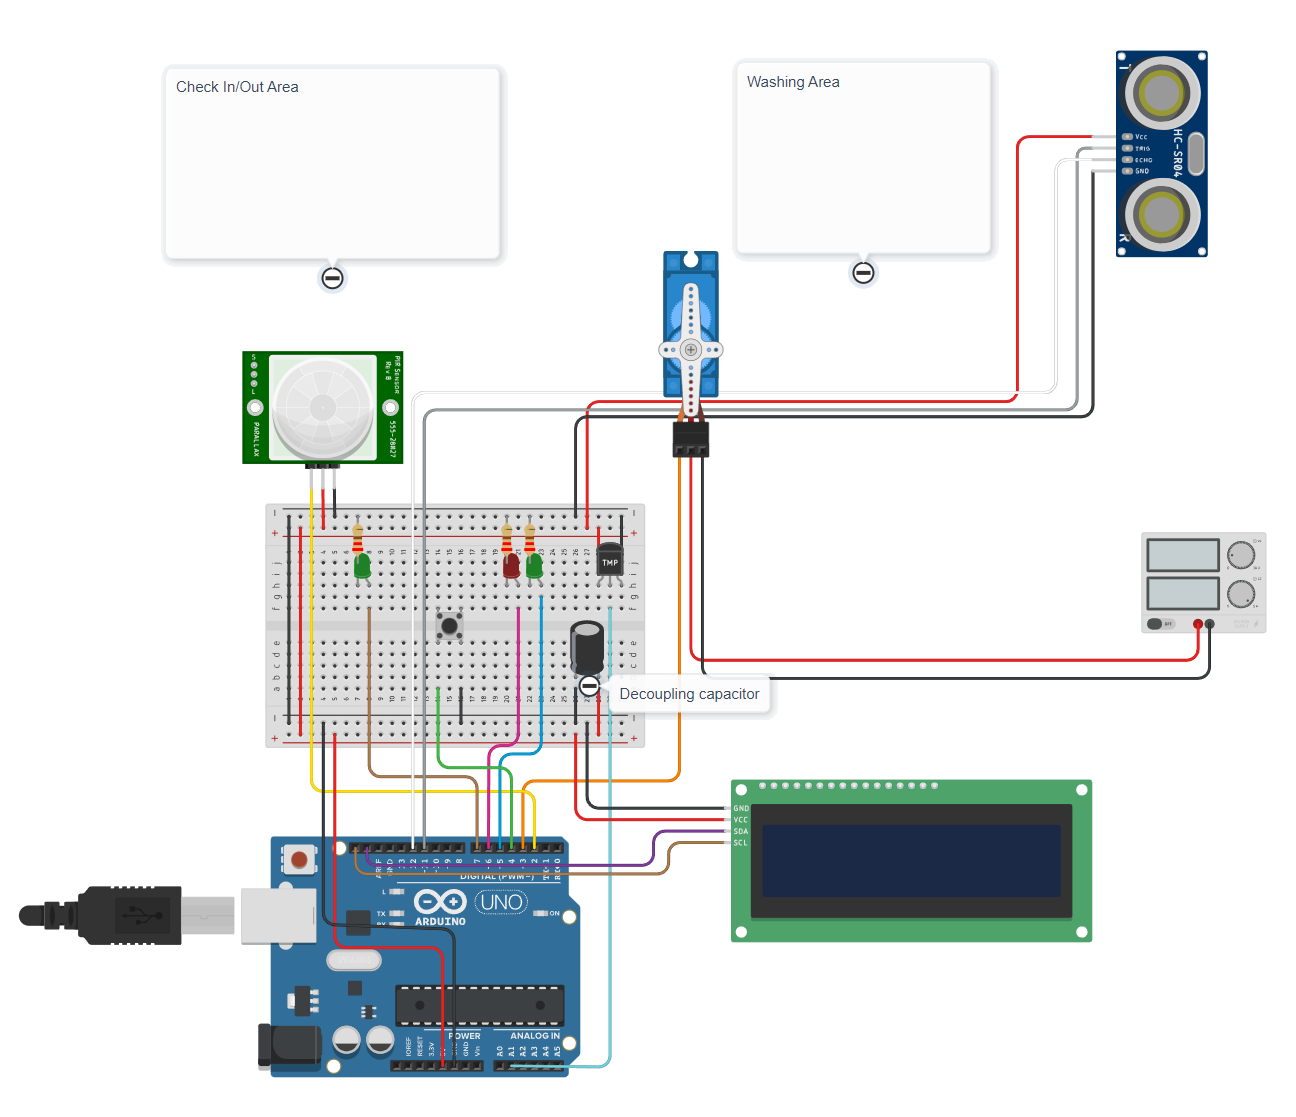
\includegraphics[width=\textwidth]{schematic}
\begin{center}
    \begin{tabular}{|c|c|}
        \hline
        Device             & pinout \\
        \hline
        \hline
        Temperature sensor & A1     \\
        \hline
        Pir                & 2      \\
        \hline
        L1                 & 7      \\
        \hline
        L2                 & 6      \\
        \hline
        L3                 & 5      \\
        \hline
        Servo              & 3      \\
        \hline
        Sonar trig         & 11     \\
        \hline
        Ssonar echo        & 12     \\
        \hline
    \end{tabular}
\end{center}
Since the servo motor might draw more current than the 150mA offered by arduino pins it's advisable to feed the servo with external power.
All the elements attached to the power line create noise that hinder the analog temperature sensor's readings.\\
To dampen this effect it is possible to add decoupling capacitors (10-100 uF) to filter a bit those variation.
\section{Software Architecture}
The program is managed by a syncronous scheduler, it is triggered by a timer and launches non cooperative tasks.\\
Each task period has been chosen accordingly to its operative requirements, and is a multiple of the base period of the scheduler.
Some empiric tests have been made to ensure that no overrun happens in any scenario.\\
The work tree of the program is divided in:\\
Sensors and actuators, containing interfaces (abstract classes) and implementations for the devices.\\
System, containing the scheduler and the task interface,\\
Task, containing all the tasks.
\section{General diagram}
\section{Tasks}
\subsection{Tasks}
\subsection{checkInDetection}

\subsection{washingAreaDetection}

\subsection{washer}
\subsection{manageTemperature}
\subsection{manageAccess}

\subsection{displayFeedback}
\subsection{communicator}
\subsection{sleepTask}

